\setchaptergraphic{
    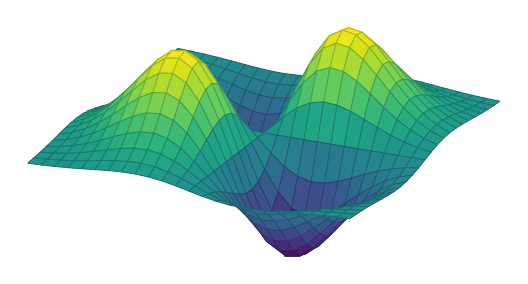
\begin{tikzpicture}[scale=0.875]
        \begin{axis}[hide axis,colormap/viridis]
            \addplot3[surf,domain=-2:2,y domain=-2:2] {7*x*y/exp(x^2+y^2)};
        \end{axis}
    \end{tikzpicture}
    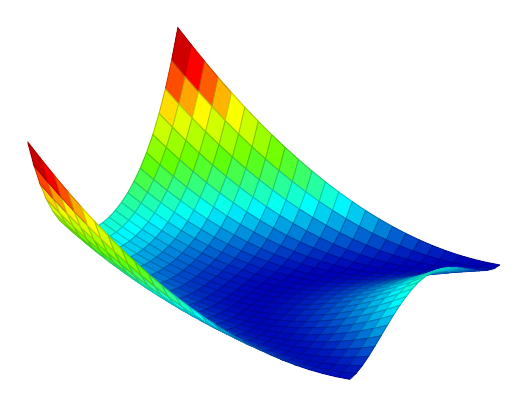
\begin{tikzpicture}[scale=0.875]
        \begin{axis}[hide axis,colormap/bluered]
            \addplot3[surf,domain=-1:1,y domain=-1:1] {(1-y)^2+100*(x-y^2)^2};
        \end{axis}
    \end{tikzpicture}
}

\chapter{Optimization}
\label{ch:optimization}

\section{Linear Programming}

\begin{defn}
    In the context of an optimization problem:
    \begin{itemize}
        \item a \emph{constraint} is a condition that needs to be satisfied,
        \item the \emph{feasible region} $S \subseteq \R^n$ is the region that satisfies all constraints,
        \item and the objective function is a function $f: S \to \R$ that is to be minimized or maximized.
    \end{itemize}
\end{defn}

\begin{figure}[ht!]
    \centering
    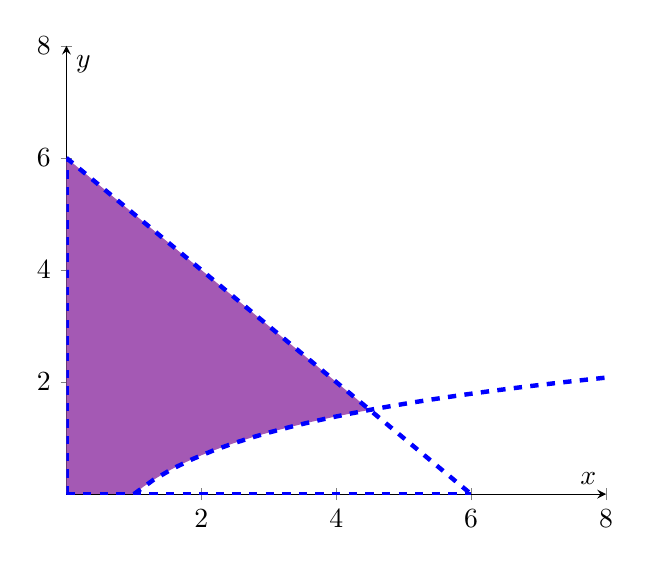
\begin{tikzpicture}[scale=1.0]
        \begin{axis}[
            axis x line=middle,
            axis y line=middle,
            ymin=0,ymax=8,ylabel=$y$,
            xmin=0,xmax=8,xlabel=$x$
        ]
            \begin{scope}
                \path[clip]
                    plot[domain=0:1] ({\x}, {0})
                    --plot[domain=1:4.49666] ({\x}, {ln(\x)})
                    --plot[domain=4.49666:0] ({\x}, {6-\x})
                    --plot[domain=0:6, variable=\y] ({0}, {\y})
                    --cycle;

                \fill [red!45!blue!65!] (0,0) rectangle (6,6);
            \end{scope}

            \plot[domain=0:6,blue,dashed,ultra thick] {6-\x};
            \plot[domain=1:8,blue,dashed,ultra thick] {ln(\x)};
            \plot[domain=0:6,blue,dashed,ultra thick] {0};
            \plot[domain=0:6,blue,dashed,ultra thick,variable=\y] ({0}, {\y});
        \end{axis}
    \end{tikzpicture}
\caption{Example feasible region (light purple) satisfying four constraints (dashed blue line)}
\label{fig:exmp-plant-feasible-region}
\end{figure}

\begin{exmp}
    Consider the problem of maximizing plant growth by manipulating quantities of two nutrients, $x_1$ and $x_2$. Let the plant height be $f(x_1, x_2) = 1 + x_1^2(x_2 - 1)^3e^{-x_1-x_2}$, with the constraints that $x_1 \geq 0$, $x_2 \geq 0$, $x_1 + x_2 \geq 6$, and $x_2 \geq \log x_1$. Then within the feasible region (depicted in Figure \ref{fig:exmp-plant-feasible-region}), $f$ is maximized by $(x_1, x_2) = (2, 4)$.
\end{exmp}

\begin{defn}
    For all $x \in \R^n$ and $\varepsilon > 0$, the \emph{$\varepsilon$-neighborhood} of $x$ is
    \[N_{\varepsilon}(x) = \left\{y \in \R^n \compbar \norm{x - y} < \varepsilon \right\}.\]
\end{defn}

\begin{exmp}
    In $\R^1$, $N_{3}(7)$ is $(4, 10)$.
\end{exmp}

\begin{defn}
    For any $S \subseteq \R^n$ and $x \in \R^n$, we say that $x$ is an \emph{interior point} of $S$ if there exists $N_{\varepsilon}(x) \subseteq S$. If every $N_{\varepsilon}(x)$ contains a point inside $S$ and a point not inside $S$, we say that $x$ is a \emph{boundary point} of $x$.
\end{defn}

\begin{defn}
    A set $S \subseteq \R^n$ is \emph{open} if every point in $S$ is an interior point of $S$, and \emph{closed} if $S$ contains every boundary point of $S$.
\end{defn}

\begin{exmp}
    In $\R^1$, any non-empty interval $[a, b]$ is closed, and non-empty $(a, b)$ is open.
\end{exmp}

\begin{exmp}
    Both $\emptyset$ and $\R^n \subseteq \R^n$ are both open and closed.
\end{exmp}

\begin{prop}
    Let $S \subseteq \R^n$. Then $S$ is open if and only if $\R^n - S$ is closed.
\end{prop}

\begin{proof}
    Assume that $S$ is open, and let $x$ be a boundary point of $\R^n - S$. Then for every $\varepsilon > 0$, by definition there exists $y, z \in N_{\varepsilon}(x)$ such that $y \in S$ and $z \in \R^n - S$. Therefore, $N_{\varepsilon}(x) \centernot\subseteq S$. It follows that $x \notin S$ by definition, and so $x \in \R^n - S$. Therefore, $\R^n - S$ contains every boundary point of itself, and so it is closed.

    Assume that $\R^n - S$ is closed, and let $x \in S$. Consider $N_{\varepsilon}(x)$. Since $\R^n - S$ contains all of its boundary points, $x$ cannot be a boundary point of $\R^n - S$, and so we know that there must be some $\varepsilon$ such that $N_{\varepsilon} \subseteq S$. Therefore, every $x \in S$ is an interior point of $S$, and so $S$ is closed by definition.
\end{proof}

\begin{exmp}
    We will examine a few cases in which minima and maxima may fail to first.

    \begin{itemize}
        \item Unbounded objective function, e.g. minimizing $\ln x$ such that $0 < x \leq 7$.
        \item Bounded objective function on open set, e.g. minimizing $\ln x$ such that $1 < x \leq 7$.
        \item Infeasible (feasible region is empty), e.g. minimizing $\ln x$ such that $1 < x$ and $x \leq 0.5$.
    \end{itemize}
\end{exmp}

\begin{exmp}
    When a solution exists, two distinct cases may occur.

    \begin{itemize}
        \item The solution is an interior point of the feasible region, e.g. minimizing $f(x) = 3 + (x - 2)^2$ such that $1 \leq x \leq 3$. The local minimum is $x^* = 2$, and $f'(x^*) = 0$.
        \item The solution is a boundary point of the feasible region, e.g. minimizing $f(x) = 3 + (x - 2)^2$ such that $x \leq 10$. Then $x^* = 10$, but $f'(x^*) \neq 0$.
    \end{itemize}
\end{exmp}

\begin{defn}
    Let $S \subseteq \R^n$ and $f: \R^n \to \R$. Consider $x^* \in S$. We say that $x^*$ is a \emph{global minimum} if for all $y \in S$, $f(x^*) \leq f(y)$, and a \emph{strict} global minimum if for all $y \in S - \{x^*\}$, $f(x^*) < f(y)$.
\end{defn}

\begin{defn}
    Let $S \subseteq \R^n$ and $f: \R^n \to \R$. Consider $x^* \in S$. We say that $x^*$ is a \emph{local minimum} if there exists an $\varepsilon$-neighborhood $N_{\varepsilon}(x^*)$ such that for all $y \in N_{\varepsilon}(x) \intersection S$, $f(x^*) \leq f(y)$, and a \emph{strict} local minimum if for all $y \in \left(N_{\varepsilon}(x) \intersection S\right) - \{x^*\}$, $f(x^*) < f(y)$.
\end{defn}

\begin{defn}
    Let $S \subseteq \R^n$ be a feasible region and $f: S \to \R$ an objective function. A \emph{stationary point} $x \in S$ is where $\nabla f(x) = \vec{0}.$
\end{defn}

\begin{rmk}
    Let $S \subseteq \R^n$, $x^*$ be an interior point of $S$, and $f: S \to \R$ be a sufficiently smooth continuous function. If $x^* \in S$ is a local minimum, then the \emph{gradient} of $f(x^*)$ is $\vec{0}$. However, $\nabla f(x^*) = \vec{0}$ does not imply that $x^*$ is a local minimum.
\end{rmk}

\subsection{Forms of Linear Programming Problems}

\begin{defn}
    A maximization or minimization linear programming problem in \emph{standard form} is a problem of the form:
    find $x \in \R^n$ that maximizes or minimizes $\transposeof{c}x$ such that $Ax = b$ and $x \geq \vec{0}$. The problem is said to be in \emph{canonical form} if the constraints are instead in the form $Ax \geq b$ (or $Ax \leq b$).
\end{defn}

\begin{exmp}
    Consider the problem of minimizing the cost per unit of chicken feed, while ensuring necessary nutrients are provided. Let $x_1, x_2, x_3, x_4$ denote the quantities of each of four ingredients, with cost per unit of $6.2$, $2.0$, $1.6$, and $3.2$ respectively. Let $n_1$, $n_2$, $n_3$ be the nutrients, with minimum required values of $6.2$, $11.9$, and $10.0$ respectively.

    \begin{minipage}{\linewidth}
        \begin{center}
        \captionof{table}{Nutrition values}
        \label{exmp-feed-nutrition-values}
        \begin{tabular}{c|cccc}
        & $x_1$ & $x_2$ & $x_3$ & $x_4$\\
        \hline
        $n_1$ & $1.2$ & $2.6$ & $0.0$ & $9.2$ \\ \hline
        $n_2$ & $3.9$ & $1.0$ & $0.8$ & $2.0$ \\ \hline
        $n_3$ & $6.0$ & $0.0$ & $4.0$ & $3.1$ \\
        \end{tabular}
        \end{center}
    \end{minipage}

    Let
    \[A = \begin{pmatrix}
        1.2 & 2.6 & 0.0 & 9.2 \\
        3.9 & 1.0 & 0.8 & 2.0 \\
        6.0 & 0.0 & 4.0 & 3.1
    \end{pmatrix},\; b = \begin{pmatrix}
        6.2 \\ 11.9 \\ 10.0
    \end{pmatrix},\; c = \begin{pmatrix}
        6.2 \\ 2.0 \\ 1.6 \\ 3.2
    \end{pmatrix},\; x = \begin{pmatrix}
        x_1 \\ x_2 \\ x_3 \\ x_4
    \end{pmatrix}\]
    then our problem is to minimize $\transposeof{c}x$ such that $Ax \geq b$ and $x \geq \vec{0}$. This form is the \emph{canonical form} of a linear programming problem.
\end{exmp}

\begin{rmk}
    We can easily convert problems expressed as a minimization problem into an equivalent maximization problem and vice versa, and between standard form and canonical form.
\end{rmk}

\begin{prop}
    Minimizing $\transposeof{c}x$ is equivalent to maximizing $-\transposeof{c}x$ (and so maximizing $\transposeof{c}x$ is equivalent to minimizing $-\transposeof{c}x$).
\end{prop}

\begin{proof}
    Let $P$ be a linear programming problem where we seek to minimize $\transposeof{c}x$, and let $S$ denote the feasible region of $P$. Now let $Q$ denote linear program where we seek to maximize $\transposeof{C}x$ that is otherwise identical to $P$. Let $x^{*}$ be a local minimum of $P$. By definition, there must exist some $\varepsilon$-neighborhood such that $\transposeof{c}x^{*} \leq \transposeof{c}y$ for all $y \in N_{\varepsilon}(x) \intersection S$. It follows that $-\transposeof{c}x^{*} \geq -\transposeof{c}y$ for all $y \in N_{\varepsilon}(x) \intersection S$, and so $x^{*}$ must be a local maximum of $Q$.
\end{proof}

\begin{prop}
    The constraint $Ax \geq b$ is equivalent to $-Ax \leq -b$, and $Ax \leq b$ is equivalent to $-Ax \geq -b$.
\end{prop}

\begin{prop}
    The constraint $Ax = b$ is equivalent to having both $Ax \geq b$ and $Ax \leq b$, and therefore is equivalent to $[A; -A] \geq [b; -b]$.
\end{prop}

\begin{prop}
    The constraint $Ax \geq b$ is equivalent to $Ax - z = b$, where $A \in M_{m \times n}(\R)$, $x \in \R^n$, and $z \in \R^m$ where $z \geq 0$. Here, $z$ is a vector of \emph{slack} variables.
\end{prop}

\begin{exmp}
    The constraints
    \begin{align*}
        a_{11}x_1 + a_{12}x_2 + a_{13}x_3 &\geq b_1 \\
        a_{21}x_1 + a_{22}x_2 + a_{23}x_3 &\geq b_2 \\
        a_{31}x_1 + a_{32}x_2 + a_{33}x_3 &\geq b_3 \\
        a_{41}x_1 + a_{42}x_2 + a_{43}x_3 &\geq b_4
    \end{align*}
    are equivalent to
    \begin{align*}
        a_{11}x_1 + a_{12}x_2 + a_{13}x_3 - x_4 &= b_1 \\
        a_{21}x_1 + a_{22}x_2 + a_{23}x_3 - x_5 &= b_2 \\
        a_{31}x_1 + a_{32}x_2 + a_{33}x_3 - x_6 &= b_3 \\
        a_{41}x_1 + a_{42}x_2 + a_{43}x_3 - x_7 &= b_4.
    \end{align*}
\end{exmp}

\begin{prop}
    We can incorporate the positivity constraints $x \geq 0$ into the general matrix constraints. The constraints $Ax \geq b$ and $x \geq 0$ are equivalent to \[\begin{bmatrix} A \\ I\end{bmatrix}x \geq \begin{bmatrix} b \\ 0 \end{bmatrix},\]
    and the constraints $Ax \leq b$ and $x \geq 0$ are equivalent to \[\begin{bmatrix} A \\ -I\end{bmatrix}x \leq \begin{bmatrix} b \\ 0 \end{bmatrix}.\]
\end{prop}

\begin{prop}
    We can transform an unconstrained problem into an equivalent problem with a positivity constraint.
\end{prop}

\begin{exmp}
    Consider the problem of minimizing $5x_1 + 6x_2$ such that $2x_1 - 3x_2 \geq 9$ and $x_1 + x_2 \geq -8$, with $x_1 \geq 0$ but $x_2$ unconstrained in sign. Define $x_2'$ and $x_2''$, and constrain $x_2', x_2'' \geq 0$. Let $x_2 = x_2' - x_2''$.
\end{exmp}

\begin{rmk}
    Constraints of the form $Ax = b$ are simply a system of equations, and therefore can be simplified using row operations by Theorem \ref{solutions-unchanged-by-row-ops}. Reduced row echelon form can help identified independent vs dependent variables.
\end{rmk}

\subsection{Polyhedrons}

\begin{defn}
    For non-zero $p \in \R^n$, the \emph{hyperplane} with normal vector $p$ is the orthogonal complement of $p$: \[\left\{x \in \R^n \compbar p \cdot x = 0 \right\},\]
    and the closed \emph{half-space} with normal vector $p$ is
    \[\left\{x \in \R^n \compbar p \cdot x \geq 0 \right\}.\]
    If we have $p \cdot x > 0$, we say it is an open half-space. We can replace $\geq$ and $>$ with $\leq$ and $<$ respectively.
\end{defn}

\begin{defn}
    A \emph{polyhedron} (or \emph{polyhedral set}) is the intersection of finitely many half spaces.
\end{defn}

\begin{defn}
    A polyhedron $P$ is \emph{bounded} if there exists $r \in \R$ such that $\norm{x} < r$ for all $x \in P$. A bounded polyhedron is known as a \emph{polytope}.
\end{defn}

\begin{prop}
    $P \subseteq \R^n$ is a polyhedron if and only if there exists $A \in M_{m \times n}(\R)$ and $b \in \R^m$ such that
    \[P = \left\{x \in \R^n \compbar Ax \geq b\right\}.\]
\end{prop}

\begin{defn}
    Let $X = \{x_1, \ldots, x_k\} \subset \R^n$. A \emph{convex combination} of $X$ is
    \[\lambda_1 x_1 + \lambda_2 x_2 + \cdots + \lambda_k x_k,\]
    where $\lambda_i \geq 0 \in \R$ and $\sum_{i=1}^{k}\lambda_i = 1$.
\end{defn}

\begin{defn}
    A set $S \subseteq \R^n$ is \emph{convex} if for any $x, y \in S$ and convex combination $z$ of $x$ and $y$, then $z \in S$.
\end{defn}

\begin{thm}
    Every polyhedron is convex.
\end{thm}

\begin{proof}
    Let $P = \left\{x \in \R^n, \compbar Ax \geq b\right\}$ be a polyhedron in $\R^n$. Let $x, y \in P$ and $z = \lambda x + (1 - \lambda) y$ be a convex combination of $x$ and $y$ for some $\lambda \in [0, 1]$.

    We know that $Ax \geq b$ and $Ay \geq b$, and want to show that $Az \geq b$. Since $z = \lambda x + (1 - \lambda)y$,
    \begin{align*}
        Az = A\left(\lambda x + (1 - \lambda)y\right) = \lambda Ax + (1 - \lambda)Ay \geq \lambda b + (1 - \lambda) b = b,
    \end{align*}
    and so $Az \geq b$.
\end{proof}

\begin{thm}
    A set $S \subseteq \R^n$ is convex if and only if every convex combination of every finite $X \subseteq S$ is in $S$.
\end{thm}

\begin{proof}
    We will prove this by showing that this is equivalent to the definition.
    
    $(\impliedby)$ If every convex combination of finite $X \subseteq S$ is in $S$, then every convex combination of $x, y \in S$ is in $X$.

    $(\implies)$ We will prove, via induction on $n = \abs{X}$, that if $z$ is a convex combination of $x, y \in S$ implies that $z \in S$, then every convex combination of $X \subseteq S$ is also in $S$.

    First, consider the base case of $n=1$, so $X = \{x\} \subseteq S$. The only convex combination of $X$ is simply $x$, and so every convex combination of $X$ is in $S$. Next, assume that if $z$ is a convex combination of $x, y \in S$ implies that $z \in S$, then every convex combination of $X \in S$ where $\abs{X} = n$ is also in $S$. For any $X' \subseteq S$ where $\abs{X'} = n+1$, there is some $X \subsetneq X'$ such that $\abs{X} = n$. Then every convex combination of $X$ is in $S$. Let \[\lambda_1x_1 + \cdots + \lambda_n x_n + \lambda_{n+1}x_{n+1}\] be a convex combination of $X$. Let $\Lambda = \lambda_1 + \cdots + \lambda_n$, and note that
    \[\alpha = \frac{\lambda_1}{\Lambda}x_1 + \cdots + \frac{\lambda_n}{\Lambda}x_n\] is a convex combination of $X$ and so must be in $S$ by by the induction hypothesis. Furthermore, note that
    \[\Lambda \alpha + \lambda_{n+1}x_{n+1}\] is our original convex combination of $X'$, but is also a convex combination of two points in $S$, and so is also in $S$ by assumption.
\end{proof}

\begin{defn}
    Let $S$ be a convex set, and consider $x \in S$. If $x$ being a convex combination of $y, z \in S$ implies that $x = y = z$, we say that $x$ is an \emph{extreme point}.
\end{defn}

\subsection{Basic Feasible Solutions}

\begin{defn}
    Let $c \in \R^n$, $A \in M_{m \times n}(\R)$, and $b \in \R^m$ be the linear program with feasibility region \[S = \left\{x \in \R^n \compbar Ax = b, x \geq \vec{0}\right\}.\] Let $A$ have rank $m$, or else eliminate redundant constraints until it does.

    Let $B$ be a subset of $m$ of the indices $\{1, \ldots, n\}$ such that the corresponding columns of $A$ form a basis for the column space of $A$ (which is $\R^m$ since $A$ has rank $m$). Let $A_B \in M_{m \times m}(\R)$ denote the invertible matrix of these columns.

    A \emph{basic feasible solution} is any $x \in S$ where $j \notin B$ implies $x_j = 0$.
\end{defn}

\begin{rmk}
    Without loss of generality, we can rearrange the columns of $A$ such that $A = [A_B | N]$, and then basic feasible solutions are precisely those $x \in S$ such that $x = \begin{bmatrix}
        x_B \\ x_N
    \end{bmatrix}$ where $x_N = \vec{0}$.
\end{rmk}

\begin{thm}
    Let $B \in M_{m \times m}(\R)$ have rank $m$, and $N \in M_{m \times (n-m)}(\R)$ where $m < n$, and then let $A = [B | N] \in M_{m \times n}(\R)$. Let $b \in \R^m$, so the feasible region is \[S = \left\{x \in \R^n \compbar Ax = b,\; x \geq \vec{0}\right\}.\]

    Then $x \in S$ is an extreme point of $S$ if and only if $x$ is a basic feasible solution of $S$.
\end{thm}

\begin{proof}\proofbreak
    ($\impliedby$) Suppose $x$ is a basic feasible solution of $S$, so $x = \begin{bmatrix}
        x_B \\ x_N
    \end{bmatrix}$ where $x_N = \vec{0}$. Let $x = \lambda x' + (1 - \lambda) x''$ be a non-trivial convex combination (so $0 < \lambda < 1$) of $x', x'' \in S$. We can represent $x'$ and $x''$ as $x' = \begin{bmatrix} x_B' \\ x_N' \end{bmatrix}$ and $x'' = \begin{bmatrix} x_B'' \\ x_N'' \end{bmatrix}$ respectively. Notice that we now have $x_N = \vec{0} = \lambda x_N' + (1 - \lambda)x_N''$. Since $x', x'' \in S$, we know $x_N', x_N'' \geq 0$ and so we necessarily have $x_N' = x_N'' = 0$. But then $x'$ and $x''$ are also basic feasible solutions. Since $A_{B}$ is invertible and $x, x', x'' \in S$, we know that $A_{B}x_B = A_{B}x_B'b = A_{B}x_B''$, and so $x = x' = x''$.

    ($\implies$) Suppose $x$ is not a basic feasible solution of $S$. Then $x = \begin{bmatrix}
        x_B \\ x_N
    \end{bmatrix}$ where $x_N$ is nonzero. We know that the columns of $A$ corresponding to the non-zero entries of $x$ must be linearly dependent, or else we can complete them to a basis for $\R^m$ and $x$ would be a basic feasible solution. Therefore, we know there exists non-zero $z$ such that $Az = \vec{0}$ and $z_i \neq 0$ implies $x_i \neq 0$. Note that for any $\alpha \in \R$, $A(x + \alpha z) = Ax + \alpha Az = b$, so any $x + \alpha z \geq \vec{0}$ is a feasible solution. Since $x_i$ is strictly greater than zero when $z_i \neq 0$, for sufficiently small $\varepsilon$ the points $x + \varepsilon z$ and $x - \varepsilon z$ must be feasible. Then $x = \frac{1}{2}\left(x + \varepsilon z\right) + \left(1 - \frac{1}{2}\right)\left(x - \varepsilon z\right)$, and so $x$ can be expressed as a non-trivial convex combination in $S$ and therefore is not extreme.
\end{proof}

\subsection{Simplex Method}

\begin{defn}
    Consider a linear program in standard form. Given a choice of basis $B$ such that $A = [B | N]$, the \emph{pre-tableau} is the matrix
    \begin{align*}
        \left[\begin{array}{c|c|c|c}
            1 & -\transposeof{c_B} & -\transposeof{c_N} & 0 \\
            \hline
            \vec{0} & B & N & b
        \end{array}\right].
    \end{align*}
    In other words, we have augment $A = [B|N]$ with the constraint values $b$, and then again with a new variable $z$ in the first column/row such that $z - \transposeof{c}x = 0$. Note that $z$ is therefore the value of the objective function.
\end{defn}

\begin{defn}
    Given a linear program in standard form, and basic feasible solution $\transposeof{x} = [\transposeof{x_B}, \vec{0}]$, the corresponding \emph{basic feasible simplex tableau} is the matrix
    \begin{align*}
        \left[\begin{array}{c|c|c|c}
            1 & 0 & \transposeof{c_B}B^{-1}N-\transposeof{c_N} & \transposeof{c_B}B^{-1}b \\
            \hline
            \vec{0} & I & B^{-1}N & B^{-1}b
        \end{array}\right].
    \end{align*}
\end{defn}

\begin{rmk}
    The basic feasible tableau is the reduced row echelon form of the pre-tableau. It can also be obtain by left-multiplying the pre-tableau by
    \begin{align*}
        \left[\begin{array}{c|c}
            1 & \transposeof{c_B}B^{-1} \\
            \hline
            \transposeof{\vec{0}} & B^{-1}
        \end{array}\right].
    \end{align*}
\end{rmk}

\begin{rmk}
    We can see that $z + (\transposeof{c_B}B^{-1}N-\transposeof{c_N})x_N = \transposeof{c_B}B^{-1}b$, so $z = \transposeof{c_B}B^{-1}b + (\transposeof{c_N} - \transposeof{c_B}B^{-1}N)x_N$. We often denote this as
    \[z = \transposeof{c_B}B^{-1}b + \transposeof{r_N}x_N,\]
    where
    \[\transposeof{r_N} = \transposeof{c_N} - \transposeof{c_B}B^{-1}N.\]
\end{rmk}

In the simplex, we start with a linear program $A, b, c$ in standard form. Assuming we already know a basis that leads to a basic feasible solution, we form the pre-tableau and either row-reduce or multiply through by the matrix from the above remark to obtain the basis feasible tableau.

To illustrate the linear program, we will consider
\begin{align*}
    A =
    \begin{bmatrix}
        2 & -1 & 3 & 7 & 1 & 2 & 8 \\
        5 & 2 & -8 & -1 & 2 & 0 & 1 \\
        4 & 6 & -2 & 4 & 1 & 3 & -5
    \end{bmatrix},\;\;
    b = \begin{bmatrix}
        2 \\ 4 \\ 3
    \end{bmatrix},\;\;
    \transposeof{c} = [6, -3, 2, 1, -1, 7, 1].
\end{align*}

We will use columns $1$, $3$, and $7$ as our basis columns, however we will leave the columns in their original order to make bookkeeping easier. Our pre-tableau is
\begin{align*}
    \left[\begin{array}{c|ccccccc|c}
        1 & -6 & 3 & -2 & -1 & 1 & -7 & -1 & 0 \\
        \hline
        0 & 2 & -1 & 3 & 7 & 1 & 2 & 8 & 2 \\
        0 & 5 & 2 & -8 & -1 & 2 & 0 & 1 & 4 \\
        0 & 4 & 6 & -2 & 4 & 1 & 3 & -5 & 3
    \end{array}\right].
\end{align*}

Row-reducing to the reduced row echelon form (while treating columns $1$, $3$, and $7$ as leading columns) brings us to our first basic feasible tableau:
\begin{align*}
    \left[\begin{array}{c|ccccccc|c}
        1 & 0 & 9.35 & 0 & 11.06 & 2.82 & -1.22 & 0 & 4.93 \\
        \hline
        0 & 1 & 1.03 & 0 & 1.62 & 0.31 & 0.82 & 0 & 0.81 \\
        0 & 0 & 0.33 & 1 & 1.14 & -0.05 & 0.50 & 0 & 0.01 \\
        0 & 0 & -0.51 & 0 & 0.04 & 0.07 & -0.14 & 1 & 0.04
    \end{array}\right].
\end{align*}

Now, we \emph{pivot} to a new (and improved!) basic feasible tableau by choosing a non-basis column to turn into a basis column. We make the greediest choice by choose the $4$th column ($5$th of the overall tableau) since it has the largest improvement to our objective function per unit change in the corresponding non-basis variable.

Letting $j = 4$, we choose the $k$th row (excluding the objective row on top) by \[\argmin_{k}\frac{b_k}{A_{kj}} \mathrm{ where } A_{kj} > 0.\] This gives us the $2$nd row, so we row-reduce again, replace the column whose leading term choose in the $2$nd row (which is column $3$) with column $4$. To do this, we treat column $4$ as if it was the second column while row-reducing. Our new basis columns are $1$, $4$, and $7$, giving us our second basic feasible tableau:
\begin{align*}
    \left[\begin{array}{c|ccccccc|c}
        1 & 0 & 6.14  & -9.67 & 0 & 3.29  & -6.01 & 0 & 4.81 \\
        \hline
        0 & 1 & 0.56  & -1.41 & 0 & 0.37  & 0.11  & 0 & 0.79 \\
        0 & 0 & 0.28  & 0.87  & 1 & -0.04 & 0.43  & 0 & 0.01 \\
        0 & 0 & -0.57 & -0.03 & 0 & 0.06  & -0.15 & 1 & 0.04
    \end{array}\right].
\end{align*}

Note that the objective function value has decreased from $4.93$ to $4.81$. We now continue pivoting in the manner, the objective function value decreasing from $4.81$, to $4.6$, to $-2.45$, to $-2.46$. When there are no positive entries in the objective function row (top row), there are no more improvements that can be made by changing our choice of basis and we have reached optimality.

\subsection{Two-Phase Method}

The Two-Phase Method is a technique for coming up with the initial basic feasible solution need to start off the Simplex Method. In Phase I, we solve a different linear program to find the initial basic feasible solution, and then in Phase II we use that basic feasible solution to apply the simplex method to the original linear program. We take a problem in standard form with constraints $Ax = b$, $x \geq 0$ where $A \in M_{m \times n}(\R)$. We then introduce \emph{artificial variables} $x_{n+1}, x_{n+2}, \ldots, x_{n+m}$ for each constraint (row) in $A$. Let $x'$ denote the vector obtained by appending the artificial variables to $x$.

For Phase I, we solve a different problem using the Simplex Method: minimizing $x_{n+1} + x_{n+2} + \cdots + x_{n+m}$ such that $[A|I]x' = b$, $x' \geq 0$. Notice that any feasible solution to this new problem is a feasible solution to the original linear program if the objective function value is zero. Therefore, the $x$ part of an optimal solution $x'$ to the new problem is a feasible solution to the original if $x'$ has objective function value zero. If the optimal solution $x'$ has a positive objective function value, then no feasible solution exists for the original linear program.

Note that
\begin{align*}
    x' = \begin{bmatrix}
        x \\
        x_{n+1} \\
        \vdots \\
        v_{n+m}
    \end{bmatrix} = \begin{bmatrix}
        0 \\
        b_1 \\
        \vdots \\
        b_m
    \end{bmatrix}
\end{align*}
is always a basic feasible solution to the Phase I problem. Therefore, we can immediately apply the Simplex method to determine the feasibility of the original linear program, and find a feasible solution if one exists. Additionally, since the number of columns in a basis for either linear program is the same (always just $m$), the feasible solution given to us by Phase I must in fact be a basic feasible solution for Phase II.

\subsection{Big-M Method}

In the Big-M method, we essentially combine the two phases of the Two-Phase method by using the objective function
\begin{align*}
    \transposeof{c}x + M(x_{n+1} + x_{n+2} + \cdots + x_{n+m}),
\end{align*}
where $M$ is a very large value. This penalizes the artificial variables and causes them to be zero in any optimal solution. Setting the artificial variables to $b$ gives us an initial basic feasible solution. If a basic feasible solution exists where the artificial variables are zero, the first $m$ pivots will replace each artificial variable with non-artificial variables, and so the final optimal solution will be a solution to the original linear program.

\subsection{Duality}

\begin{defn}{Canonical or symmetric duality}\proofbreak
    Consider a linear program of the form minimize $\transposeof{c}x$ such that $Ax \geq b$ and $x \geq \vec{0}$. The \emph{dual} problem is maximizing $\transposeof{b}y$ such that $\transposeof{A}y \leq c$ and $y \geq \vec{0}$. The original linear program is referred to as the \emph{primal} probem in relation to its dual.
\end{defn}

\begin{exmp}
    Consider minimizing $1x_1 + 2x_2$ such that
    \begin{align*}
        3x_1 + 4x_2 &\geq 9, \\
        5x_1 + 6x_2 &\geq 10, \\
        7x_1 + 8x_2 &\geq 11, \\
        x_1, x_2 &\geq 0.
    \end{align*}

    The dual problem is maximizing $9y_1 + 10y_2 + 11y_3$ such that
    \begin{align*}
        3y_1 + 5y_2 + 7y_3  &\leq 1, \\
        4y_1 + 6y_2 + 8y_3  &\leq 2, \\
        y_1, y_2, y_3 &\geq 0.
    \end{align*}
\end{exmp}

\begin{defn}{Standard duality}\proofbreak
    Consider a linear program of the form minimization of $\transposeof{c}x$ such that $Ax = b$ and $x \geq \vec{0}$. The \emph{dual} problem is maximizing $\transposeof{b}y$ such that $\transposeof{A}y \leq c$, \emph{without} a non-negativity constraint on $y$. The original linear program is again referred to as the \emph{primal} probem in relation to its dual.
\end{defn}

\begin{rmk}
    We can derive the canonical form of duality from the standard form, and vice versa. Imagine we know that the dual of minimizing $\transposeof{c}x$ such that $Ax = b$ and $x \geq \vec{0}$ was to maximize $\transposeof{b}y$ such that $\transposeof{A}y \leq c$. If we were now given a linear program in canonical form and wanted to find its dual, we could first convert it into standard form by the introduction of slack variables, obtaining minimize $\transposeof{c}x$ such that $[A|-I]\begin{bmatrix}x \\ z\end{bmatrix} = b$ such that $\begin{bmatrix}x \\ z\end{bmatrix} \geq 0$. The standard dual of this is to maximize $\transposeof{b}y$ such that $\transposeof{[A|-I]}y \leq \begin{bmatrix}c \\ \vec{0}\end{bmatrix}$, which is equivalent to maximizing $\transposeof{b}y$ such that $\transposeof{A}y \leq c$ and $y \geq \vec{0}$ (from $-y \leq \vec{0}$).
\end{rmk}

\begin{prop}
    The canonical and standard duals of equivalent linear programs are equivalent.
\end{prop}

\begin{proof}
    See figure \ref{fig:duality-equivalence}.
\end{proof}

\begin{figure}[ht]
    \centering
    \begin{tikzpicture}[{baseline=(current bounding box.north)}]
        \node[align=center] at (-3,2.5) {$
            \begin{aligned}
                \mathrm{min.}\;\transposeof{c}&x \\
                \mathrm{s.t.}\;A&x \geq b, \\
                        &x \geq \vec{0}.
            \end{aligned}
        $};
        \node[align=center] at (3,2.5) {$
            \begin{aligned}
                \mathrm{max.}\;\transposeof{b}&y \\
                \mathrm{s.t.}\;\transposeof{A}&y \leq c, \\
                        &y \geq \vec{0}.
            \end{aligned}
        $};
        \node[align=center] at (-3,-3) {$
            \begin{aligned}
                \mathrm{min.}\;\transposeof{\begin{bmatrix}c \\ \vec{0}\end{bmatrix}}&\begin{bmatrix}x \\ z\end{bmatrix} \\
                \mathrm{s.t.}\;\left[A|-I\right]&\begin{bmatrix}x \\ z\end{bmatrix} = b, \\
                        &x, z \geq \vec{0}.
            \end{aligned}
        $};
        \node[align=center] at (3,-3) {$
            \begin{aligned}
                \mathrm{max.}\;&\transposeof{b}y \\
                \mathrm{s.t.}\;&\begin{bmatrix}\transposeof{A} \\ -I\end{bmatrix}y \leq \begin{bmatrix}c \\ \vec{0}\end{bmatrix}.
            \end{aligned}
        $};

        \draw[ultra thick, blue, ->] (-1, 3) -- (1, 3);
        \draw[ultra thick, red, ->] (-1, -3) -- (1, -3);
        \draw[ultra thick, black, <->] (3, -1) -- (3, 1);
        \draw[ultra thick, black, <->] (-3, 1) -- (-3, -1);

    \end{tikzpicture}
\caption{Equivalence of dualities}
\label{fig:duality-equivalence}
\end{figure}

\newpage

\begin{prop}
    Given a primal linear program, the dual of the dual is the primal.
\end{prop} 

\begin{proof}
    Consider a linear program in canonical form.  By definition, the dual is maximizing $\transposeof{b}y$ such that $\transposeof{A}y \leq c$ and $y \geq 0$. This program is equivalent to minimizing $-\transposeof{b}y$ such that $-\transposeof{A}y \geq -c$ and $y \geq 0$. The dual of this equivalent form of the dual is to maximizing $-\transposeof{c}x$ such that $\transposeof{\left(-\transposeof{A}\right)}x \leq -b$ and $x \geq 0$. Finally, this program is equivalent to minimizing $\transposeof{c}x$ such that $Ax \geq b$ and $x \geq 0$, which is the primal linear program.
\end{proof}

\begin{thm}{Weak Duality}\label{weak-duality}\proofbreak
    Consider a linear program and its dual, and $x, y$ feasible solutions to the primal and dual programs respectively. Then the objective function value at $y$ in the dual is less than or equal to the objective function value at $x$ in the primal.
\end{thm}

\begin{proof}
    When the primal is in standard form, we have $Ax = b$, $x \geq \vec{0}$ and $\transposeof{A}y \leq c$. It follows that $\transposeof{b}y = \transposeof{(Ax)}y = \transposeof{x}\transposeof{A}y$. Since we have $x \geq \vec{0}$, we know that $\transposeof{x}\transposeof{A}y \leq \transposeof{x}c$, and so $\transposeof{b}y \leq \transposeof{c}x$.

    When the primal is in canonical form, we have $Ax \geq b$, $x \geq \vec{0}$, $\transposeof{A}y \leq c$, and $y \geq 0$. Since $y \geq \vec{0}$, $Ax \geq b$ implies that $\transposeof{b}y \leq \transposeof{(Ax)}y$, and so $\transposeof{b}y \leq \transposeof{x}\transposeof{A}y$. Furthermore, since $\transposeof{A}y \leq c$ and $x \geq \vec{0}$, $\transposeof{x}\transposeof{A}y \leq \transposeof{x}c = \transposeof{c}x$. Combining these, we arrive at $\transposeof{b}y \leq \transposeof{c}y$.
\end{proof}

\begin{cor}
    The optimal objective value function in the dual is less than or equal to the optimal objective function value in the primal.
\end{cor}

\begin{cor}{Supervisor principle}\label{supervisor-principle}\proofbreak
    If $\transposeof{b}y = \transposeof{c}x$, then $x$ and $y$ are optimal in their respective linear programs.
\end{cor}

\begin{thm}{Strong Duality}\label{strong-duality}\proofbreak
    Suppose a linear program has a feasible solution and its objective function is bounded from below. Then the linear program and its dual have optimal solutions $x$ and $y$ respectively, and the objective function value of $x$ and $y$ are equal.
\end{thm}

\begin{proof}
    Consider the primal in standard form. We can apply the Simplex method or similar to obtain an optimal basic feasible solution $x^*$. Without loss of generality, we can assume that the final basis consists of the first $m$ columns of $A$.

    By the terminating condition of the Simplex method, we know that
    \begin{align*}
        \transposeof{r_N} = \transposeof{c_N} - \transposeof{c_B}B^{-1}N \geq \vec{0}.
    \end{align*}
    Let
    \begin{align*}
        \transposeof{y^*} = \transposeof{c_B}B^{-1}.
    \end{align*}

    Since $\transposeof{r_N} \geq \vec{0}$, we know that
    \begin{align*}
        \transposeof{c_B}B^{-1}N \leq \transposeof{c_N},
    \end{align*}
    and so it follows that
    \begin{align*}
        \transposeof{y^*}A = \transposeof{c_B}B^{-1}[B|N] = [\transposeof{c_B}|\transposeof{c_B}B^{-1}N] \leq [\transposeof{c_B}|\transposeof{c_N}] = \transposeof{c},
    \end{align*}
    so $y^*$ is a feasible solution to the dual. Now we can show that the objective function values are equal:
    \begin{align*}
        \transposeof{y^*}b = \transposeof{c_B}B^{-1}b = \transposeof{\begin{bmatrix}c_B \\ \vec{0}\end{bmatrix}}\begin{bmatrix}x_B \\ \vec{0}\end{bmatrix} = \transposeof{c}x^*.
    \end{align*}

    Therefore, $y^*$ is an optimal solution to the dual linear program by the supervisor principle \ref{supervisor-principle}.
\end{proof}

\begin{defn}
    A basic feasible solution $b$ to a linear program with basis $B$ is \emph{non-degenerate} when $B^{-1}b > \vec{0}$.
\end{defn}

Consider solving a linear program $A, b, c$ in standard form by the Simplex method. What happens if we replace $b$ with $b' = b + \Delta b$ for some arbitrary $\Delta b$? If we replaced $B^{-1}b$ with $B^{-1}(b + \Delta b)$ and $\transposeof{c_B}B^{-1}b$ with $\transposeof{c_B}B^{-1}(b + \Delta b)$ in just the final basic feasible simplex tableau, what happens?

If $B^{-1}(b + \Delta b) \geq \vec{0}$, then we still have a basic feasible solution! Furthermore, since the objective row would still be non-positive, our solution would also be an \emph{optimal} basic feasible solution. This would very likely only occur when $\Delta b$ is fairly small.

If the linear program is non-degenerate, there always exists such $\Delta b$ small enough.

In the corresponding dual linear program, we know that
\begin{align*}
    \transposeof{y^*} = \transposeof{c_B}B^{-1}.
\end{align*}
We also have $\transposeof{c}x^* = \transposeof{y^*}b$, and so when we replace $b$ with $b'$ we get
$\transposeof{c}{x'}^{*} = \transposeof{y^*}(b + \Delta b) = \transposeof{y^*}b + \transposeof{y^*}\Delta b$. Therefore,
\begin{align*}
    \frac{\partial\transposeof{c}{x}^{*}}{\partial b_i} = y_i^*.
\end{align*}

\begin{defn}
    Vectors $x, y \in \R^n$ are \emph{complementary} if $x_i \neq 0 \implies y_i = 0$ and $y_i \neq 0 \implies x_i = 0$.
\end{defn}

\begin{prop}\label{complementary-orthogonal}
    If $x \geq 0$ and $y \geq 0$, then $x$ and $y$ are complementary if and only if $\transposeof{x}y = 0$.
\end{prop}

\begin{proof}
    If $x$ and $y$ are complementary, then $x_iy_i = 0$, and so $\transposeof{x}y = 0$.

    Since $x \geq 0$ and $y \geq 0$, we know $x_iy_i \geq 0$. If $\transposeof{x}y = 0$, then we must have $x_iy_i = 0$. Therefore at least one of $x_i$ and $y_i$ is zero and so $x$ and $y$ are complementary.
\end{proof}

\begin{thm}{Complementary slackness}\label{complementary-slackness}\proofbreak
    Consider a linear program $A, b, c$ in standard form. Let $x \in \R^n$ be a feasible solution. Let $y \in \R^m$ be a feasible solution in the dual. Then $x$ and $y$ are optimal solutions if and only if $c - \transposeof{A}y$ is complentary to $x$.
\end{thm}

\begin{proof}
    Recall that
    \begin{align*}
        \transposeof{b}y = \transposeof{(Ax)}y = \transposeof{x}\transposeof{A}y \leq \transposeof{x}c = \transposeof{c}x.
    \end{align*}
    By the supervisor principle \ref{supervisor-principle}, $x$ and $y$ are optimal if and only if $\transposeof{b}y = \transposeof{c}x$, which is equivalent to $\transposeof{x}\transposeof{A}y = \transposeof{x}c$. Therefore,
    \begin{align*}
        \transposeof{x}\left(c - \transposeof{A}y\right) = \vec{0}.
    \end{align*}

    Since $y$ is feasible in the dual, by definition $\transposeof{A}y \leq c$, and so $c - \transposeof{A}y \geq \vec{0}$. Furthermore, $x \geq 0$ and so by Proposition \ref{complementary-orthogonal} it follows that this occurs precisely when $x$ and $c - \transposeof{A}y$ are complementary.
\end{proof}

\subsection{Dual Simplex Method}

In the dual simplex method, we have a linear program in standard form. Unlike when we start the simplex method, rather than knowing a starting feasible solution and working towards optimality, we know a starting solution that is essentially optimal and works towards feasibility. We actually start with a vector $y$ that is feasible in the dual linear program, and work towards making the corresponding primal vector $x$ feasible in the primal. Due to the setup of the dual simplex method, both $y$ and $x$ will have the same objective function value, and so once $x$ is feasible we have an optimal solution by the supervisor principle \ref{supervisor-principle}.

\begin{defn}{Basic tableau}\proofbreak
    A basic tableau is a tableau formed from a basic, but not necessarily feasible, solution.
\end{defn}

Given a linear program in standard form and corresponding basic tableau, we have $\transposeof{y} = \transposeof{c_B}B^{-1}$ and $x = B^{-1}b$. Recall that $y$ is an optimal solution to the dual problem when:
\begin{itemize}
    \item $Ax = b$,
    \item $x \geq 0$,
    \item $\transposeof{A}y \leq c$,
    \item $\transposeof{c}x = \transposeof{b}y$.
\end{itemize}

The first condition, that $Ax = b$ is necessarily satisfied by any basic tableau. The fourth, that $\transposeof{c}x = \transposeof{b}y$, is also satisfied since $\transposeof{c_B}B^{-1}b = \transposeof{y}b = \transposeof{b}y$ and $\transposeof{c_B}B^{-1}b = \transposeof{c}x$. The third condition, that $\transposeof{A}y \leq c$, is satisfied when $r \geq 0$. Since the top row of the tableau is $-r$, to have dual feasibility at the start of the dual simplex method we require that $-r \leq 0$ --- that is, that the top row of the basic tableau is non-positive other than the constant $1$. Therefore, we need to come up with a ``dual pivot'' that preserves these properties while working towards achieving the second condition.

To dual pivot, we choose the row $j$ with the most-negative value in $B^{-1}b$, and pick a column to row-reduce on. Since we need to maintain a non-positive top row $-r$, we want to pick the column $k$ by \[\argmin_{k}\frac{r_k}{A_{jk}} \mathrm{ where } A_{jk} < 0.\]

\section{Non-Linear Programming}

\begin{defn}
    Let $S \subseteq \R^n$ be a non-empty convex set, and let $f: S \to \R$. We say that $f$ is \emph{convex} when
    \begin{align*}
        f\left(\lambda x + (1 - \lambda)y\right) \leq \lambda f(x) + (1 - \lambda)f(y)
    \end{align*}
    for all $x, y \in S$ and $\lambda \in [0, 1]$.

    Similarly, we say that $f$ is \emph{strictly convex} when
    \begin{align*}
        f\left(\lambda x + (1 - \lambda)y\right) < \lambda f(x) + (1 - \lambda)f(y)
    \end{align*}
    for all $x, y \in S$ and $\lambda \in (0, 1)$.

    We analogously define \emph{concave} and \emph{strictly concave} functions using $\geq$ and $>$ respectively.
\end{defn}

\begin{rmk}
    Note that we use an open interval for $\lambda$ in the strict case, and a closed interval otherwise. This is because at $\lambda = 0$ or $\lambda = 1$ we will always have equality.
\end{rmk}

\begin{defn}
    Let $S \subseteq \R^n$, and consider $f: S \to \R$. The \emph{epigraph} of $f$ 
    \begin{align*}
        \left\{\begin{bmatrix}
            x \\ y
        \end{bmatrix} \compbar x \in S, y \in R, y \geq f(x)\right\} \subseteq \R^{n+1}
    \end{align*}
    and is denoted by $\epigraphof{f}$. That is, the epigraph is all points above the graph of the function.
\end{defn}

\begin{prop}\label{epigraph-convexity}
    Let $S \subseteq \R^n$, and consider $f: S \to \R$. Then $f$ is a convex function if and only if $\epigraphof{f}$ is a convex set.
\end{prop}

\begin{proof}\proofbreak
    ($\implies$) Assume that $f$ is convex. Then for any $\transposeof{[x_1, y_1]}, \transposeof{[x_2, y_2]} \in \epigraphof{f}$ and $\lambda \in [0, 1]$, we know that
    \begin{align*}
        f(\lambda x_1 + (1 - \lambda)x_2) \leq \lambda f(x_1) + (1 - \lambda)f(x_2) \leq \lambda y_1 + (1 - \lambda)y_2.
    \end{align*}
    Therefore,
    \begin{align*}
        \lambda \begin{bmatrix}
            x_1 \\ y_1
        \end{bmatrix} + (1-\lambda)\begin{bmatrix}
            x_2 \\ y_2
        \end{bmatrix} = \begin{bmatrix}
            \lambda x_1 + (1 - \lambda)x_2 \\
            \lambda y_1 + (1 - \lambda)y_2
        \end{bmatrix} \in \epigraphof{f},
    \end{align*}
    and so $\epigraphof{f}$ is a convex set.

    ($\impliedby$) Assume that $\epigraphof{f}$ is a convex set. Since we trivially have $f(x) \leq f(x)$ for all $x \in S$, we know that for any $x_1, x_2 \in S$ we have
    \begin{align*}
        \transposeof{[x_1, f(x_1)]}, \transposeof{[x_2, f(x_2)]} \in \epigraphof{f}.
    \end{align*}
    Since $\epigraphof{f}$ is convex, for all $\lambda \in [0, 1]$ we also know that
    \begin{align*}
        \lambda \begin{bmatrix}
            x_1 \\ f(x_1)
        \end{bmatrix} + (1-\lambda)\begin{bmatrix}
            x_2 \\ f(x_2)
        \end{bmatrix} = \begin{bmatrix}
            \lambda x_1 + (1 - \lambda)x_2 \\
            \lambda f(x_1) + (1 - \lambda)f(x_2)
        \end{bmatrix} \in \epigraphof{f}.
    \end{align*}
    Therefore,
    \begin{align*}
        f(\lambda x_1 + (1 - \lambda)x_2) \leq \lambda f(x_1) + (1-\lambda)f(x_2)
    \end{align*}
    by the definition of $\epigraphof{f}$, and so $f$ is a convex function.
\end{proof}

\begin{thm}{Support Theorem}\label{support-theorem}\proofbreak
    Let $S \subseteq \R^n$ be a convex set, and let $\bar{x}$ be a boundary point of $S$. There exists a hyperplane containing $\bar{x}$ such that $S$ is contained in an associated closed half-space.
\end{thm}

\begin{thm}\label{convex-function-tangent-hyperplane}
    Let $S \subseteq \R^n$ be an open convex set, and let $f: S \to \R$ be continuously differentiable. Then $f$ is a convex function if and only if
    \begin{align*}
        f(x) \geq f(\bar{x}) + \transposeof{\nabla f(\bar{x})}(x - \bar{x})
    \end{align*}
    for all $x, \bar{x} \in S$. 
\end{thm}

\begin{thm}
    Let $S \subseteq \R^n$ be an open convex set, and let $f: S \to \R$ be \emph{twice} continuously differentiable. Then $f$ is convex if and only if $\nabla^2f(\bar{x})$ is positive semi-definite for all $\bar{x} \in S$.
\end{thm}

\begin{proof}\proofbreak
    Assume $\nabla^2f(\bar{x})$ is positive semi-definite for all $\bar{x} \in S$. By Taylor's theorem, for all $x \in S$ we have
    \begin{align*}
        f(x) = f(\bar{x}) + \transposeof{\nabla f(\bar{x})}(x - \bar{x}) + \frac{1}{2}\transposeof{(x - \bar{x})}\nabla^2f(z)(x - \bar{x})
    \end{align*}
    for some $z \in S$. Since $\nabla^2f(\bar{x})$ is positive semi-definite, we know that $\frac{1}{2}\transposeof{(x - \bar{x})}\nabla^2f(z)(x - \bar{x}) \geq 0$, and so we have
    \begin{align*}
        f(x) \geq f(\bar{x}) + \transposeof{\nabla f(\bar{x})}(x - \bar{x}).
    \end{align*}

    Now assume $\nabla^2f(\bar{x})$ is \emph{not} positive semi-definite for all $\bar{x} \in S$. Then there exists $d \in \R^n$ such that $\transposeof{d}\nabla^2f(\bar{x})d < 0$. By continuity of $\nabla^2f(\bar{x})$, there is a neighborhood around $\bar{x}$ such that $\transposeof{d}\nabla^2f(z)d < 0$ for all $z$ in that neighborhood. By Taylor's theorem, for all $x \in S$ we have
    \begin{align*}
        f(x) = f(\bar{x}) + \transposeof{\nabla f(\bar{x})}(x - \bar{x}) + \frac{1}{2}\transposeof{(x - \bar{x})}\nabla^2f(z)(x - \bar{x})
    \end{align*}
    for some $z \in S$. Choose $x = \bar{x} + \alpha d$ for $\alpha > 0$ small enough that $x$ is in that neighborhood, and since $z$ falls between $x$ and $\bar{x}$, $z$ is also in that neighborhood. Then $\frac{1}{2}\transposeof{(x - \bar{x})}\nabla^2f(z)(x - \bar{x}) < 0$, and so we have
    \begin{align*}
        f(x) < f(\bar{x}) + \transposeof{\nabla f(\bar{x})}(x - \bar{x}).
    \end{align*}
\end{proof}

\begin{prop}
    Let $S \in \R^n$ be an open convex set, and let $f: S \to \R$ be a continuously differentiable convex function. Then for any $\bar{x} \in S$, the following are equivalent:
    \begin{itemize}
        \item $\bar{x}$ is a global minimum,
        \item $\bar{x}$ is a local minimum,
        \item $\bar{x}$ is stationary point.
    \end{itemize}
\end{prop}

\begin{proof}
    If $\bar{x}$ is a global minimum, then $\bar{x}$ is a local minimum. If $\bar{x}$ is a local minimum, then $\bar{x}$ is a stationary point. Therefore, we only need to show that stationary points are global minimums, and the result will follow.

    By convexity of $f$, for all $x \in S$ we know that $f(x) \geq f(\bar{x}) + \transposeof{\nabla f(\bar{x})}(x - \bar{x})$ by Theorem \ref{convex-function-tangent-hyperplane}. If $\bar{x}$ is a stationary point, then $\nabla f(\bar{x})$ by definition, and so $f(x) \geq f(\bar{x})$. Then $\bar{x}$ is a global minimum by definition.
\end{proof}

\begin{defn}{Newton's Method}\label{newtons-method}\proofbreak
    Let $f: \R^n \to \R$ be twice continuously differentiable, and pick some $x^{(0)} \in \R^n$. For $i = 1, 2, \ldots, $ while $\nabla f(x^{(i)}) \neq 0$ (or until some other terminating condition), let
    \begin{align*}
        x^{(i+1)} = x^{(i)} - \left(\nabla^2f(x^{(i)})\right)^{-1}\nabla f(x^{(i)}).
    \end{align*}
\end{defn}

\begin{rmk}
    Assume that $\nabla^2f$ is constant, and that all derivatives of $f$ of order higher than two are zero. Then a local minimum occurs when $\nabla f(x) = 0$, and so we want $\nabla f(x^{(i+1)}) = 0$. Since the higher derivatives are zero,
    \begin{align*}
        \nabla f(x^{(i+1)}) = \nabla f(x^{(i)}) + \nabla^2f(x^{(i)})(x^{(i+1)} - x^{(i)}).
    \end{align*}
    Therefore, if we want the gradient to be zero, we have
    \begin{align*}
        0 &= \nabla f(x^{(i)}) + \nabla^2f(x^{(i)})(x^{(i+1)} - x^{(i)}) \\
        x^{(i+1)} - x^{(i)} &= -\left(\nabla^2f(x^{(i)})\right)^{-1}\nabla f(x^{(i)}) \\
        x^{(i+1)} &= x^{(i)} - \left(\nabla^2f(x^{(i)})\right)^{-1}\nabla f(x^{(i)}).
    \end{align*}
    While our assumptions will almost certainly be invalid, making these ``Newton steps'' will often produce rapid progress towards a local minimum. For non-pathological functions, the closer to the local minimum the better our linear approximation of $\nabla f$ will be.
\end{rmk}

\begin{defn}{Steepest Descent}\label{steepest-method}\proofbreak
    Let $f: \R^n \to \R$ be continuously differentiable, and pick some $x^{(0)} \in \R^n$. 
    For $i = 1, 2, \ldots, $ while $\nabla f(x^{(i)}) \neq 0$ (or until some other terminating condition), define
    \begin{align*}
        g(\alpha) = f(x^{(i)} - \alpha\nabla f(x^{(i)})),
    \end{align*}
    and then let
    \begin{align*}
        \alpha^* &= \argmin_{\alpha}g(\alpha) \\
        x^{(i+1)} &= x^{(i)} - \alpha^{*}\nabla f(x^{(i)}).
    \end{align*}
\end{defn}

\subsection{Karush-Kuhn-Tucker Conditions}

\begin{thm}{Farkas' Theorem}\label{farkas}\proofbreak
    Let $A \in M_{m \times n}(\R)$, $b \in \R^m$. Then exactly one of the following is true:
    \begin{itemize}
        \item there exists $x \in \R^n$ such that $Ax = b$ and $x \geq \vec{0}$,
        \item there exists $y \in \R^m$ such that $\transposeof{b}y > 0$ and $\transposeof{A}y \leq \vec{0}$.
    \end{itemize}
\end{thm}

\begin{proof}
    Consider the linear program of minimizing $\transposeof{\vec{0}}x$ such that $Ax = b$ and $x \geq {0}$. The dual program is maximizing $\transposeof{b}y$ such that $\transposeof{A}y \leq \vec{0}$.

    In the first case, the primal program is feasible and the objective function value at $x$ is necessarily zero. Then by Weak Duality \ref{weak-duality}, we know that the dual program has no feasible solution with objective function value greater than zero, and so the second case cannot be true.

    If the second case is false, then the dual program has no feasible solutions with positive objective function value. We know however that the $y = \vec{0}$ is a feasible solution to the dual with objective function value of zero, and is therefore the optimal solution. By Strong Duality \ref{strong-duality}, the primal program must have a feasible solution $x$, and so the first case is true.
\end{proof}

\begin{thm}{Gordon's Theorem}\label{gordons}\proofbreak
    Let $A = M_{m \times n}(\R)$. Then exactly one of the following is true:
    \begin{itemize}
        \item there exists $x \in \R^n$ such that $Ax = \vec{0}$, $x \geq \vec{0}$, $x \neq \vec{0}$.
        \item there exists $y \in \R^m$ such that $\transposeof{A}y < \vec{0}$.
    \end{itemize}
\end{thm}

\begin{proof}
    Assume the second case is true, so there exists $y \in \R^m$ such that $\transposeof{A}y < \vec{0}$. Equivalently, there exists $\varepsilon > 0$ such that $\transposeof{A}y + \varepsilon\vec{1} \leq \vec{0}$ --- that is, there exists
    \begin{align*}
        \begin{bmatrix}
            y \\ \varepsilon
        \end{bmatrix} \in \R^{m+1}
    \end{align*}
    such that
    \begin{align*}
        \transposeof{\begin{bmatrix}
            \vec{0} \\ 1
        \end{bmatrix}}
        \begin{bmatrix}
            y \\ \varepsilon
        \end{bmatrix} > 0,\;\;\;\begin{bmatrix}
            \transposeof{A} | \vec{1}
        \end{bmatrix}\begin{bmatrix}
            y \\ \varepsilon
        \end{bmatrix} \leq \vec{0}.
    \end{align*}
    By Farkas \ref{farkas}, this is true if and only if there is no $x \geq \vec{0}$ such that
    \begin{align*}
        \begin{bmatrix}
            A \\ \transposeof{\vec{1}}
        \end{bmatrix}x = \begin{bmatrix}
            \vec{0} \\ 1
        \end{bmatrix}.
    \end{align*}
    This is in turn equivalent to
    \begin{align*}
        Ax = \vec{0},\;\;\;x \geq \vec{0}\;\;\;\transposeof{\vec{1}}x = 1.
    \end{align*}
    Note that this is equivalent to the first case from this theorem: the existence of $x \neq 0$ implies the existence of
    \begin{align*}
        x' = \frac{1}{\transposeof{\vec{1}}x}x,
    \end{align*}
    and we would have $Ax' = \frac{1}{\transposeof{\vec{1}}x}\vec{0} = \vec{0}$, $x' \geq \vec{0}$, $\transposeof{\vec{1}}x' = 1$. Conversely, if $x = \vec{0}$ then $\transposeof{\vec{1}}x = \vec{0}$, so if $\transposeof{\vec{1}}x = 1$, then $x \neq \vec{0}$.

    Therefore, the second case is equivalent to the negation of the first, and so exactly one of them is true for any $A$.
\end{proof}

\begin{rmk}
    From here until the Karush-Kuhn-Tucker Conditions, let $P$ be the problem of minimizing $f(x)$ such that $g_i(x) \leq 0$ for $i = 1, \ldots, m$ where $f: \R^n \to \R$ and $g_i: \R^n \to \R$ are continuously differentiable.
\end{rmk}

\begin{defn}
    For all feasible $x \in \R^n$, the \emph{active constraints} at $x$ are
    \begin{align*}
        \mathcal{A}_x = \left\{i \compbar g_i(x) = 0\right\}.
    \end{align*}
\end{defn}

\begin{defn}
    For a function $f: \R^n \to \R$ and point $x_0 \in \R^n$, a vector $d \in \R^n$ is a \emph{descent direction} if there exists $\alpha_0 > 0$ such that $f(x + \alpha d) < f(x)$ for all $0 < \alpha \leq \alpha_0$.
\end{defn}

\begin{lemma}\label{kkt-lemma-1}
    If $x$ is a local minimum of $P$ (and therefore feasible), then there \emph{does not} exist $d \in \R^n$ that is a descent direction for $f(x)$ and for $g_i(x)$ for all $i \in \mathcal{A}_x$. 
\end{lemma}

\begin{proof}
    If such $d$ existed, then there would exist $\varepsilon > 0$ small enough that $f(x + \alpha d) < f(x)$ and $g_i(x + \alpha d) < g_i(x) = 0$ for $i \in \mathcal{A}_x$. For $i \notin \mathcal{A}_x$, we know that $g_i(x) < 0$ and so for $\varepsilon$ small enough we also have $g_i(x + \alpha d) < 0$. Then $x + \alpha d$ would be feasible, and so $x$ would not be a local minimum.
\end{proof}

\begin{lemma}\label{kkt-lemma-2}
    Let
    \begin{align*}
        \transposeof{J} = \begin{bmatrix}
            \nabla \transposeof{f}(x) \\ \nabla \transposeof{g_{k_1}}(x) \\ \vdots \\ \nabla \transposeof{g_{k_n}}(x)
        \end{bmatrix}
    \end{align*}
    for all $k_i \in \mathcal{A}(x)$.

    If $x$ is a local minimum of $P$, then there \emph{does not} exist $d \in \R^n$ such that $\transposeof{J}d < \vec{0}$.
\end{lemma}

\begin{proof}
    If such $d$ existed, then it would be a descent direction for $f$ and $g_{k_i}$ since $\nabla \transposeof{f}(x)d = \nabla f(x) \cdot d$ and $\nabla \transposeof{g_{k_i}}(x)d = \nabla g_{k_i}(x) \cdot d$. Therefore, no such $d$ exists by Lemma \ref{kkt-lemma-1}
\end{proof}

\begin{lemma}\label{kkt-lemma-3}
    If $x$ is a local minimum of $P$, then there exists non-zero $\lambda \geq \vec{0}$ such that $J\lambda = \vec{0}$.
\end{lemma}

\begin{proof}
    By Lemma \ref{kkt-lemma-2}, there is no $d$ such that $\transposeof{J}d < \vec{0}$. Therefore, by Gordon's Theorem \ref{gordons}, there must be $\lambda \geq 0$, $\lambda \neq \vec{0}$ such that $J\lambda = \vec{0}$.
\end{proof}

\begin{lemma}\label{kkt-lemma-4}
    If $x$ is a local minimum of $P$, then there exists non-zero
    \begin{align*}
        \begin{bmatrix}
            \beta \\ \lambda
        \end{bmatrix} \geq \vec{0}
    \end{align*}
    where $\beta \in \R$ and $\lambda \in \R^m$ such that
    \begin{align*}
        \left[\begin{array}{c|c|c|c|c}
            \nabla f(x) & \nabla g_1(x) & \nabla g_2(x) & \vdots & \nabla g_m(x)
        \end{array}\right]\begin{bmatrix}
            \beta \\ \lambda
        \end{bmatrix} = \vec{0},\;\;\textrm{and}\;\sum_{i=1}^{n}\lambda_ig_i(x) = 0.
    \end{align*}
\end{lemma}

\begin{proof}
    Since $g_i(x) \leq 0$ and $\lambda_i \geq 0$, it follows from
    \begin{align*}
        \sum_{i=1}^{n}\lambda_ig_i(x) = 0
    \end{align*}
    that $\lambda_i = 0$ whenever $g_i(x) \neq 0$, or else the sum would be less than zero. Therefore, we can ignore the columns inactive constaints, and this result follows from Lemma \ref{kkt-lemma-3}.
\end{proof}

\begin{thm}{Fritz-John Conditions}\label{fritz-john-conditions}\proofbreak
    If $x$ is a local minimum of $P$, then there exists $\lambda \in \R^m$ and $\beta \in \R$ such that
    \begin{align*}
        \beta\nabla f(x) + \nabla \vec{g}(x)\lambda = \vec{0} \\
        \transposeof{\lambda}\vec{g}(x) = 0 \\
        \lambda \geq \vec{0},\;\beta \geq 0 \\
        \begin{bmatrix}
            \beta \\ \lambda
        \end{bmatrix} \neq \vec{0}.
    \end{align*}
\end{thm}

\begin{proof}
    This is equivalent to Lemma \ref{kkt-lemma-4}.
\end{proof}

\begin{thm}{Karush-Kuhn-Tucker Conditions}\label{kkt-conditions}\proofbreak
    Let $x$ be a (necessarily feasible) local minimum of $P$. Suppose $x$ satisfies the constraint qualification that
    \begin{align}
        \left\{\nabla g_i(x) \compbar i \in \mathcal{A}_x\right\}
    \end{align}
    is linearly independent. Then there exists $\lambda \in \R^m$ such that
    \begin{align*}
        \nabla f(x) + \nabla \vec{g}(x)\lambda = \vec{0}, \\
        \transposeof{\lambda}\vec{g}(x) = 0, \\
        \lambda \geq \vec{0}.
    \end{align*}
\end{thm}

\begin{proof}
    We can apply the Fritz-John Conditions \ref{fritz-john-conditions} to obtain $\beta$ and $\lambda_0$. Since $\nabla g_i(x)$ are linearly independent, it follows that $\nabla g_i(x)\lambda_0 \neq \vec{0}$. Therefore, $\beta \neq 0$. Let $\lambda = \frac{1}{\beta}\lambda_0$. Then
    \begin{align*}
        \nabla f(x) + \nabla \vec{g}(x)\lambda = \vec{0},
    \end{align*}
    and the other conditions follow directly from the Fritz-John conditions.
\end{proof}

\begin{exmp}
    Consider the problem of minimizing $f(x, y) = x^2 + y^2$ such that $x \geq 1$ (that is, $g(x, y) = 1 - x \leq 0$), and imagine we want to find all KKT points and their multipliers. Note that
    \begin{align*}
        \nabla f\begin{bmatrix}
            x \\ y
        \end{bmatrix} = \begin{bmatrix}
            2x \\ 2y
        \end{bmatrix},\;\;
        \nabla g\begin{bmatrix}
            x \\ y
        \end{bmatrix} = \begin{bmatrix}
            -1 \\ 0
        \end{bmatrix}.
    \end{align*}

    Note that since $\nabla g \neq \vec{0}$, the KKT constraint qualification is always satisfied. Therefore, any optimal point must satisfy the KKT conditions. We can consider two separate cases: when $g$ is active or inactive. When $g$ is inactive, $g(x, y) < 0 \implies x > 1$, and also $\lambda = 0$. Therefore, any optimal point must satisfy
    \begin{align*}
        \nabla f(x, y) + \nabla g(x, y)\lambda = \vec{0} \implies \nabla f(x, y) = \vec{0}.
    \end{align*}
    However, this is impossible when $x > 1$. Therefore, any optimal point can only occur when the constraint $g$ is active, so $x = 1$. Then there must exist $\lambda$ such that
    \begin{align*}
        \nabla f(x, y) + \nabla g(x, y)\lambda = \vec{0} \implies \begin{bmatrix}
            2 \\ y
        \end{bmatrix} + \lambda \begin{bmatrix}
            -1 \\ 0
        \end{bmatrix} = \vec{0},
    \end{align*}
    which of course implies that $\lambda = 2$, and so $y = 0$. Therefore, the only KKT point is $(1, 0)$, and so it must be optimal.
\end{exmp}

\begin{exmp}
    Consider the problem of minimizing $f(x, y) = \frac{x^2}{2} + \frac{y^2}{2}$ such that $g(x, y) = 1 + x + y \leq 0$, and imagine we want to find all KKT points and their multipliers. Note that
    \begin{align*}
        \nabla f\begin{bmatrix}
            x \\ y
        \end{bmatrix} = \begin{bmatrix}
            x \\ y
        \end{bmatrix},\;\;
        \nabla g\begin{bmatrix}
            x \\ y
        \end{bmatrix} = \begin{bmatrix}
            1 \\ 1
        \end{bmatrix}.
    \end{align*}
    If $(x, y)$ is feasible, then either $g$ is active or not. If $g$ is inactive, then the constraint qualification is vacously satisfied. Then $(x, y)$ is not a KKT point, since the KKT conditions are only satisfied at $(0, 0)$ which is infeasible. So KKT points can only occur when $g$ is active, and so $y = -x - 1$. Then the KKT conditions state that
    \begin{align*}
        \begin{bmatrix}
            x \\ -x - 1
        \end{bmatrix} + \lambda\begin{bmatrix}
            1 \\ 1
        \end{bmatrix} = \begin{bmatrix}
            0 \\ 0
        \end{bmatrix},
    \end{align*}
    and so we have $\lambda = -x$ and $\lambda = x + 1$, so $2x + 1 = 0$. It follows that $x = -\frac{1}{2}$ and so $\lambda = \frac{1}{2}$ and $y = -\frac{1}{2}$.
\end{exmp}

\begin{exmp}
    Let $A \in M_{n\times n}(\R)$ be symmetric and positive definite, $b \in \R^n$ be non-zero, and $c \in \R$ be positive. Consider the problem of minimizing $f(x) = \frac{1}{2}\transposeof{x}Ax$ such that $g(x) = \transposeof{b}x + c \leq 0$. Imagine we want to find all KKT points and their multipliers. Note that
    \begin{align*}
        \nabla f(x) = Ax,\;\;
        \nabla g(x) = b.
    \end{align*}
    For any feasible $x$, we know that $g$ is either active or inactive. If $g$ is inactive, then the constraint qualification is vacously satisfied and so $Ax = \vec{0}$. Since $A$ is positive definite, $x = \vec{0}$, which is infeasible since $c > 0$. Therefore, $g$ must be active. Note that since $b$ is non-zero, the constraint qualification is satisfied. Therefore, we want to find feasible $x$ such that
    \begin{align*}
        Ax + \lambda b = \vec{0},
    \end{align*}
    for $\lambda \geq 0$. We then have $x = -\lambda A^{-1}b$. For $x$ to be feasible and $g$ be active, we need $\transposeof{b}\left(-\lambda A^{-1}b\right) + c = \vec{0}$ and so the only KKT multiplier and point is
    \begin{align*}
        \lambda = \frac{c}{\transposeof{b}A^{-1}b},\;\; x = -\frac{c}{\transposeof{b}A^{-1}b}A^{-1}b.
    \end{align*}
\end{exmp}

\begin{exmp}
    Consider the linear program of minimizing $\transposeof{c}x$ such that $Ax \geq b$ and $x \geq 0$. Alternatively, minimize $f(x) = \transposeof{c}x$ such that
    \begin{align*}
        \vec{g}(x) = \begin{bmatrix}
            -A \\ -I
        \end{bmatrix}x + \begin{bmatrix}
            b \\ \vec{0}
        \end{bmatrix} \leq \vec{0}.
    \end{align*}
    Imagine we want to find all KKT points and their multipliers. Note that
    \begin{align*}
        \nabla f(x) = c,\;\;
        \nabla \vec{g}(x) = \begin{bmatrix}
            -\transposeof{A} | -\transposeof{I}
        \end{bmatrix}.
    \end{align*}
    The constraint qualification requires that $A$ is full row-rank, we can always reduce $A$ if that is not the case. Therefore, we can safely assume that the constraint qualification is always satisfied. The KKT conditions are then
    \begin{align*}
        c + \begin{bmatrix}
            -\transposeof{A} | -\transposeof{I}
        \end{bmatrix}\begin{bmatrix}
            y \\ z
        \end{bmatrix} = \vec{0} \\
        \begin{bmatrix}
            \transposeof{y} | \transposeof{z}
        \end{bmatrix}\left(\begin{bmatrix}
            -A \\ -I
        \end{bmatrix}x + \begin{bmatrix}
            b \\ \vec{0}
        \end{bmatrix}\right) = 0 \\
        \begin{bmatrix}
            y \\ z
        \end{bmatrix} \geq \vec{0}.
    \end{align*}
    It follows that
    \begin{align*}
        \transposeof{A}y + z &= c, \\
        \transposeof{y}Ax &= \transposeof{y}b = \transposeof{b}y, \\
        \transposeof{z}x &= 0.
    \end{align*}
    Therefore, $z = c - \transposeof{A}y$, and so $\transposeof{z}x = 0$ implies that $\transposeof{c}x = \transposeof{b}y$ and $z \geq \vec{0}$ implies that $\transposeof{A}y \leq c$. Altogether, the KKT conditions then require that
    \begin{align*}
        Ax &\geq b, \;\; x \geq \vec{0}, \\
        \transposeof{A}y &\leq c, \;\; y \geq \vec{0},
    \end{align*}
    and $\transposeof{c}x = \transposeof{b}y$. Notice that these are equivalent to the requirements for complementary slackness \ref{complementary-slackness}.
\end{exmp}

\begin{thm}\label{convex-KKT-sufficiency}
    Let $S \subseteq \R^n$ be a non-empty open convex set, and let $f: S \to \R$ and $g_i: S \to \R$ be continuously differentiable and convex for $i = 1, \ldots, m$. Consider the linear program where we seek to minimize $f(x)$ such that $g_i(x) \leq 0$. For any $x \in S$, if there exists $\lambda \in \R^m$ such that
    \begin{align*}
        \nabla f(x) + \nabla \vec{g}(x)\lambda = \vec{0}, \\
        \transposeof{\lambda}\vec{g}(x) = 0, \\
        \lambda \geq \vec{0},
    \end{align*}
    then $x$ is a global minimum.
\end{thm}

\begin{rmk}
    This theorem says that if $f$ and $g_i$ are convex and continuously differentiable, then the KKT conditions, without needing the constraint qualification, are sufficient for global optimality.
\end{rmk}

\begin{cor}
    If $f, g_i$ are not globally convex, but have positive definite Hessians at some feasible $\bar{x}$, then $\bar{x}$ being a KKT point is sufficient for $\bar{x}$ to be a local minimum.
\end{cor}
